\documentclass[11pt,a4paper]{article}

% ---------- Packages ----------
\usepackage[utf8]{inputenc}
\usepackage[T1]{fontenc}
\usepackage{lmodern}
\usepackage{amsmath,amssymb,siunitx,booktabs}
\usepackage{enumitem}
\usepackage{geometry}
\usepackage{fancyhdr}
\usepackage[most]{tcolorbox}   % enhanced, breakable
\usepackage{hyperref}

% ---------- Geometry ----------
\geometry{margin=2.5cm}

% ---------- Header/Footer ----------
\setlength{\headheight}{14pt}  % fancyhdr warning verhindern
\pagestyle{fancy}
\fancyhf{}
\lhead{Einführung in die Elektrotechnik}
\rhead{Wintersemester 2025}
\cfoot{\thepage}

% ---------- Exercise Environment ----------
\newcounter{exercise}
\newenvironment{exercise}[1][]
  {\refstepcounter{exercise}%
   \begin{tcolorbox}[enhanced, breakable, width=\textwidth,
     colback=blue!5!white,colframe=blue!60!black,
     fonttitle=\bfseries\large,
     title=Aufgabe~\theexercise:~#1]}
  {\end{tcolorbox}}

% ---------- Solution Environment ----------
\newif\ifshowsolutions
\showsolutionstrue  % comment to hide solutions

\newenvironment{solution}
  {\ifshowsolutions
     \begin{tcolorbox}[enhanced, breakable, width=\textwidth,
       colback=green!5!white,colframe=green!50!black,
       fonttitle=\bfseries\large,
       title=Lösung]}
  {\end{tcolorbox}\fi}

% ---------- Document ----------
\begin{document}

% ----- Header Box -----
\begin{tcolorbox}[enhanced, breakable, colback=gray!10!white,
  colframe=gray!70!black, fonttitle=\bfseries\large,
  title={Aufgabenblatt \#8}: AC Power and Resonances, sharp corners, width=\textwidth]
\begin{center}
  Besprechung: 15.12.2025
\end{center}
\end{tcolorbox}
\vspace{1cm}

% ----- Exercise 1 -----
\begin{exercise}[Momentan- und Durchschnittsleistung]
Gegeben sind $v(t)=160\cos(50t)\,\text{V}$ und $i(t)=-33\sin(50t-30^\circ)\,\text{A}$. Berechne die momentane Leistung und die Durchschnittsleistung.
\end{exercise}

\ifshowsolutions
\begin{solution}
Zunächst wird der Strom umgeschrieben mit der Identität
\[
\sin x = \cos(x-90^\circ):
\]
\[
i(t)=-33\cos\!\big[(50t-30^\circ)-90^\circ\big] = -33\cos(50t-120^\circ).
\]

Die Momentanleistung ist
\[
p(t) = v(t)i(t) =160\cos(50t)\,\big[-33\cos(50t-120^\circ)\big] = -5280\cos(50t)\cos(50t-120^\circ).
\]

Benutzung der Identität
\[
\cos A \cos B = \tfrac12\left[\cos(A-B)+\cos(A+B)\right].
\]

Mit \(A = 50t\), \(B = 50t-120^\circ\):
\[
p(t) = -5280 \cdot \tfrac12\left[\cos\big(120^\circ\big)+\cos\big(100t-120^\circ\big)\right] = -2640\left[\cos 120^\circ + \cos(100t-120^\circ)\right].
\]

Da \(\cos 120^\circ = -\tfrac12\),
\[
p(t) = -2640\left[-\tfrac12 + \cos(100t -120^\circ)\right] = 1320 - 2640\cos(100t-120^\circ).
\]

Somit gilt für die **Momentanleistung**:
\[
\boxed{p(t)=1320 + 2640\cos(100t+60^\circ)\ \text{W}}.
\]

Die **Durchschnittsleistung** ist der DC-Anteil:
\[
\boxed{\overline{P} = 1320\ \text{W}}.
\]
\end{solution}
\fi

% ----- Exercise 2 -----
\begin{exercise}[Komplexe Leistungsberechnung]
Für den gesamten unten abgebildeten Schaltkreis berechne:
\begin{enumerate}[label=\alph*)]
  \item die komplexe Leistung
  \item die durchschnittliche Leistung (Wirkleistung), die von der Quelle geliefert wird
  \item die Blindleistung
  \item die Scheinleistung
  \item den Leistungsfaktor
\end{enumerate}

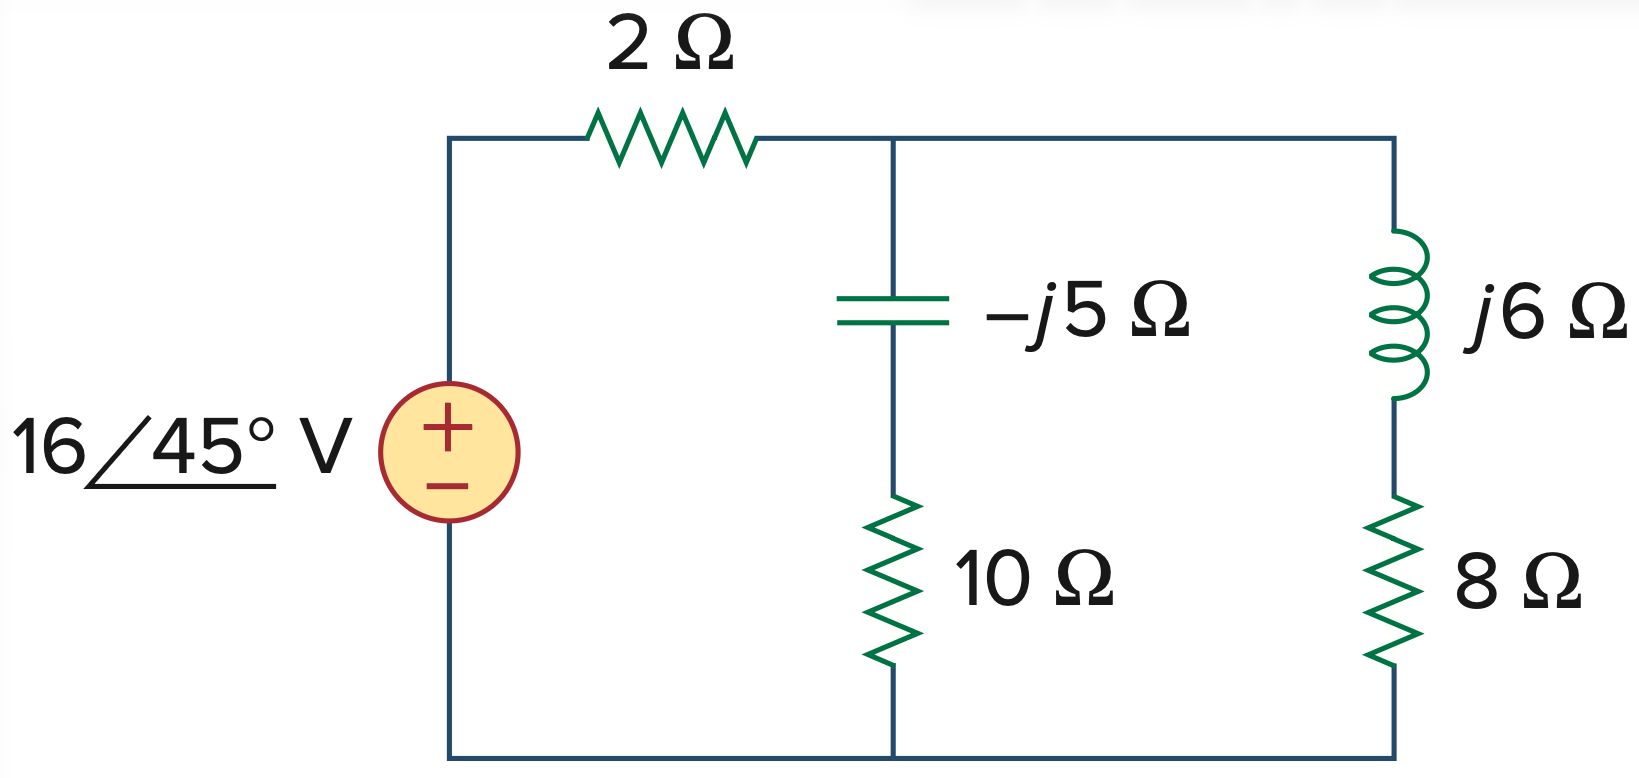
\includegraphics[width=0.7\textwidth]{figures/complex_power.png}
\end{exercise}

\ifshowsolutions
\begin{solution}
Zwei parallele Zweige nach dem 2\(\Omega\) Widerstand:
\[
\underline{Z}_1 = 10 - j5,\qquad \underline{Z}_2 = 8 + j6.
\]

Gesamtimpedanz (inklusive des 2\(\Omega\) Widerstands in Serie):
\[
\underline{Z} = 2 + \left(\frac{1}{\underline{Z}_1} + \frac{1}{\underline{Z}_2}\right)^{-1} = 2 + \Big(\frac{1}{10-j5} + \frac{1}{8+j6}\Big)^{-1}
\]
\[
= 2 + \Big(\frac{10+j5}{100+25} + \frac{8-j6}{64+36}\Big)^{-1} = 2 + \Big(0.08 + j0.04 + 0.08 - j\,0.06\Big)^{-1}
\]
\[
= 2 + \frac{0.16 + j\,0.02}{0.16^2 + 0.02^2} = 2 + \frac{0.16 + j\,0.02}{0.026} = \frac{0.212 + j\,0.02}{0.026}\,\Omega
\]
\[
Z = \frac{\sqrt(0.212^2 + 0.02^2)}{0.026} \approx 8.1901\,\Omega
\]
\[
\varphi = \arctan\!\frac{0.02}{0.212} = 5.39^\circ
\]

Quellspannung (komplexer Effektivwert als Phasor):
\[
\underline{V}_s = 16 \cdot e^{j\,45^\circ} = (11.3137 + j\,11.3137)\,\text{V}
\]
Quellstrom (komplexer Effektivwert als Phasor):
\[
\underline{I}_s = \frac{\underline{V}_s}{\underline{Z}} = \frac{16}{8.1901} \cdot e^{j\,(45^\circ - 5.39^\circ)} = 1.9536 \cdot e^{j\,39.61^\circ} = (1.5051 + j\,1.2455)\,\text{A}
\]

\begin{enumerate}[label=\alph*)]
\item Komplexe Leistung der Quelle:
\[
\underline{S} = \underline{V}_s \underline{I}_s^* = (11.3137 + j\,11.3137)\,\text{V} \cdot (1.5051 - j\,1.2455)\,\text{A} = (31.12 + j\,2.94)\,\text{VA}.
\]

\item Wirkleistung der Quelle:
\[
P = \text{Re}(\underline{S}) = 31.12\,\text{W}
\]

\item Blindleistung:
\[
Q = \text{Im}(\underline{S}) = 2.94\,\text{VAR}
\]

\item Scheinleistung:
\[
S = \sqrt{P^2 + Q^2} = 31.26\,\text{VA}.
\]

\item Leistungsfaktor (Skalar) und Typ:
\[
\cos \varphi = \dfrac{P}{S} = \dfrac{31.12}{31.26} \approx 0.9956.
\]
Da \(Q>0\) ist die Last induktiv, also \emph{nachlaufend}.
\end{enumerate}
\end{solution}
\fi

% ----- Exercise 3 -----
\begin{exercise}[Effektivwerte und Durchschnittsleistung]
Die Spannung über einer Last und der Strom durch sie sind gegeben durch
$v(t)=20+60\cos(100t)\,\text{V}$ and $i(t)=1-0.5\sin(100t)\,\text{A}$.
Bestimme:
\begin{enumerate}[label=\alph*)]
  \item die Effektivwerte der Spannung und des Stroms
  \item die durchschnittliche Leistung, die in der Last umgesetzt wird
\end{enumerate}
\end{exercise}

\ifshowsolutions
\begin{solution}
\begin{enumerate}[label=\alph*)]
\item Für ein Signal, das aus einem konstanten (DC) Anteil und einer einzelnen Sinuswelle besteht,
\[
x(t) = X_{\mathrm{DC}} + \hat{x} \cos(\omega t+\phi),
\]
ist das mittlere Quadrat (Zeitmittelwert von \(x^2(t)\)) über eine Periode
\[
\overline{x^2(t)} = X_{\mathrm{DC}}^2 + \frac{\hat{x}^2}{2},
\]
weil der Kreuzterm zwischen DC- und Sinusanteil zu null gemittelt wird und der Sinusanteil \(\hat{x}^2/2\) beiträgt. Der Effektivwert ist somit
\[
X = \sqrt{X_{\mathrm{DC}}^2 + \dfrac{\hat{x}^2}{2}}.
\]

Anwenden auf die Spannung:
\[
V_{\mathrm{DC}} = 20,\qquad \hat{v} = 60
\]
Somit gilt
\[
V = \sqrt{20^2 + \frac{60^2}{2}} = \sqrt{2200} = 10\sqrt{22} \approx 46.9\,\text{V}.
\]

Anwenden der gleichen Formel auf den Strom ergibt
\[
i(t) = I_{\mathrm{DC}} + \hat{i} \cos(100t + \phi_i),
\]
wobei \(I_{\mathrm{DC}} = 1\). Der Wechselstromanteil ist \(-0.5 \sin(100t)\) mit Amplitude \(\hat{i} = 0.5\). (Das Vorzeichen und die Phase beeinflussen den Effektivwert nicht.) Somit gilt
\[
I = \sqrt{1^2 + \frac{(0.5)^2}{2}} = \sqrt{1.125} \approx 1.061\,\text{A}.
\]

\item Die Momentanleistung beiträgt
\[
p(t) = v(t) i(t) = (20 + 60 \cos(100t))\bigl(1 - 0.5 \sin(100t)\bigr).
\]
Ausmultiplizieren ergibt:
\[
p(t) = 20 \cdot 1 + 20 \cdot (-0.5 \sin(100t)) + 60 \cos(100t) \cdot 1 + 60 \cos(100t) \cdot (-0.5 \sin(100t))
\]
\[
= 20 - 10 \sin(100t) + 60 \cos(100t) - 30 \cos(100t) \sin(100t)
\]
Die Durchschnittsleistung ist der zeitliche Mittelwert von \(p(t)\) über eine Periode. Jeder reine Sinus (oder das Produkt von Sinusfunktionen gleicher Frequenz, das zu einem Sinus mit doppelter Frequenz reduziert wird) hat einen Mittelwert von null. Somit ist der zeitliche Mittelwert von \(-10 \sin(100t)\), von \(60 \cos(100t)\) und von \(-30 \cos(100t) \sin(100t)\) jeweils null. Daher bleibt nur der DC-Anteil übrig:
\[
P = \overline{p(t)} = 20\,\text{W}
\]

Alternativ kann man die Durchschnittsleistung auch mit der Zerlegung in DC- und Sinusanteile berechnen:
\[
P = V_{\mathrm{DC}}I_{\mathrm{DC}} + \frac{1}{2} \hat{v} \hat{i} \cos\varphi,
\]
wobei \(\varphi\) der Phasenunterschied zwischen Spannungs- und Stromsinus ist. Hier ist \(V_{\mathrm{DC}} I_{\mathrm{DC}} = 20 \cdot 1\) und der sinusförmige Anteil hat
\[
\hat{v} = 60,\qquad \hat{i} = 0.5.
\]
Spannung: \(60 \cos(100t)\) (phase \(0\)). Strom: \(-0.5 \sin(100t) = 0.5 \cos(100t + \tfrac{\pi}{2})\) (Phase \(+\tfrac{\pi}{2}\)). Somit gilt \(\varphi = 0 - (+\tfrac{\pi}{2}) = -\tfrac{\pi}{2}\) und \(\cos\varphi = \cos(-\tfrac{\pi}{2}) = 0\). Demnach ist der sinusförmige Beitrag null und
\[
P = 20\,\text{W}.
\]
\end{enumerate}
\end{solution}
\fi

% ----- Exercise 4 -----
\begin{exercise}[Blindleistungskompensation]  
Ein Gleichstrommotor mit der Impedanz $\underline{Z} = 4.2 + j\,3.6\,\Omega$ wird von einer 220-V, 60-Hz Quelle gespeist.
\begin{enumerate}[label=\alph*)]
  \item Bestimme den Leistungsfaktor, die Wirkleistung P und die Blindleistung Q.
  \item Berechne die Kapazität des Kondensators, der parallel zum Motor geschaltet werden muss, damit der Leistungsfaktor auf Eins korrigiert wird.
\end{enumerate}
\end{exercise}

\ifshowsolutions
\begin{solution}
\begin{enumerate}[label=\alph*)]
\item Die Größe und der Winkel der Lastimpedanz sind
\[
|\underline{Z}| = \sqrt{R^2 + X^2} = \sqrt{4.2^2 + 3.6^2} \approx 5.532\,\Omega,
\]
\[
\varphi = \arctan\!\frac{X}{R} = \arctan\!\frac{3.6}{4.2} \approx 0.709\,\text{rad} \approx 40.6^\circ.
\]

Der Effektivwert des Stroms ist
\[
I = \frac{V}{|\underline{Z}|} = \frac{220}{5.532} \approx 39.77\,\mathrm{A}.
\]

Der Leistungsfaktor ist der Kosinus des Impedanzwinkels (nachlaufend, da \(X>0\)):
\[
\cos \varphi \approx 0.76\quad\text{(lagging)}.
\]

Berechne die komplexe Leistung:
\[
\underline{S} = \frac{V^2}{\underline{Z}^*} = V^2/(R - jX)^* = \frac{V^2(R + jX)}{R^2 + X^2}
\]

Damit sind Wirk- und Blindleistung
\[
P = \frac{V^2 R}{R^2 + X^2} \approx 6.643\,\mathrm{kW},
\]
\[
Q = \frac{V^2 X}{R^2 + X^2} \approx 5.694\,\mathrm{kVAR}.
\]

\item Um den Leistungsfaktor auf Eins zu korrigieren, muss eine kapazitive Blindleistung \(Q_C\) bereitgestellt werden, die die induktive Blindleistung \(Q\) des Motors aufhebt. Für einen Kondensator, der parallel über die gleiche Effektivspannung \(V\) geschaltet ist, gilt
\[
|Q_C| = V^2 \,\omega C,\qquad \omega = 2\pi f.
\]

Wir brauchen \( |Q_C| = Q \), also
\[
C = \frac{Q}{V^2 \omega} = \frac{5694}{220^2 \cdot 2\pi \cdot 60} \approx 312\,\mu\mathrm{F}.
\]
\end{enumerate}
\end{solution}
\fi

% ----- Exercise 5 -----
\begin{exercise}[Serienschwingkreis]
Eine serielle RLC-Schaltung hat $R = \SI{2}{\kilo\ohm}$, $L = \SI{40}{\milli\henry}$ und $C = \SI{1}{\micro\farad}$. Berechne die Impedanz bei Resonanz und bei einem Viertel, der Hälfte, dem Doppelten und dem Vierfachen der Resonanzfrequenz.
\end{exercise}

\ifshowsolutions
\begin{solution}
Für eine serielle RLC-Schaltung mit
\[
R=\SI{2}{\kilo\ohm},\qquad L=\SI{40}{\milli\henry},\qquad C=\SI{1}{\micro\farad}
\]
ist die Serienimpedanz
\[
\underline{Z}(j\omega)=R+j\bigl(\omega L-\tfrac{1}{\omega C}\bigr).
\]

Resonanz tritt auf, wenn die Netto-Reaktanz null ist:
\[
\omega_0=\frac{1}{\sqrt{LC}}
\]
Einsetzen der Werte ergibt:
\[
\omega_0=\frac{1}{\sqrt{(40\times10^{-3})(1\times10^{-6})}}=\SI{5000}{\radian\per\second}
\]

Für eine gegebene Kreisfrequenz \(\omega\) gilt:
\[
X_L=\omega L,\qquad X_C=\frac{1}{\omega C},\qquad X=X_L-X_C,
\]
\[
\underline{Z} = R + jX,\qquad |\underline{Z}| = \sqrt{R^2 + X^2},\qquad \varphi = \arctan\!\frac{X}{R}.
\]

Wir berechnen für \(\omega = k\omega_0\) mit \(k=\tfrac14,\tfrac12,1,2,4\).

\bigskip
\begin{tabular}{@{}lcccccc@{}}
\toprule
$k$ & $\omega$ (rad/s) & $X_L$ (\si{\ohm}) & $X_C$ (\si{\ohm}) & $\underline{Z}$ (\si{k\ohm}) & $|\underline{Z}|$ (\si{k\ohm}) & $\varphi$ \\
\midrule
$0.25$ & $1250$ & $50$ & $800$ & $2 - j0.75$ & $2.136$ & $-20.6^\circ$ \\[4pt]
$0.5$ & $2500$ & $100$ & $400$ & $2 - j0.3$ & $2.022$ & $-8.5^\circ$ \\[4pt]
$1$ & $5000$ & $200$ & $200$ & $2$ & $2$ & $0^\circ$ \\[4pt]
$2$ & $10000$ & $400$ & $100$ & $2 + j0.3$ & $2.022$ & $+8.5^\circ$ \\[4pt]
$4$ & $20000$ & $800$ & $50$ & $2 + j0.75$ & $2.136$ & $+20.6^\circ$ \\
\bottomrule
\end{tabular}

\bigskip
\noindent Observations:
\begin{itemize}
  \item Bei Resonanz ($\omega=\omega_0$) heben sich die induktive und kapazitive Reaktanz auf, so dass eine rein ohmsche Impedanz \(Z=R=\SI{2000}{\ohm}\) verbleibt.
  \item Für Frequenzen unterhalb der Resonanz ($k<1$) ist die Netzreaktanz kapazitiv ($X<0$), für Frequenzen oberhalb der Resonanz ($k>1$) ist sie induktiv ($X>0$).
  \item Die Impedanzen treten in konjugierten Paaren für reziproke Frequenzverhältnisse auf (z.B. für \(k=\tfrac14\) und \(k=4\); \(k=\tfrac12\) und \(k=2\)).
\end{itemize}
\end{solution}
\fi

% ----- Exercise 6 -----
\begin{exercise}[Parallelschwingkreis]
Bearbeite Aufgabe 6 erneut, wenn die Elemente parallel geschaltet sind.
\end{exercise}

\ifshowsolutions
\begin{solution}
Für die Parallelschaltung ist die Gesamtadmittanz
\[
\underline{Y}(j\omega) = \underbrace{\frac{1}{R}}_{G} + j\Bigl(\underbrace{\omega C}_{B_C} + \underbrace{\Bigl(-\frac{1}{\omega L}\Bigr)}_{B_L}\Bigr) = G + jB(\omega).
\]
Die Impedanz ist der Kehrwert der Admittanz:
\[
\underline{Z}(\omega) = \frac{1}{\underline{Y}(\omega)} = \frac{1}{G+jB} = \frac{G-jB}{G^2+B^2}
\]
Ihre Größe und Phase sind
\[
|\underline{Z}|=\frac{1}{\sqrt{G^2+B^2}},\qquad \varphi = \operatorname{atan2}\bigl(\Im\{Z\},\Re\{Z\}\bigr) = \arctan\!\frac{-B}{G}.
\]

Parallelresonanz (Netto-Suszeptanz null) tritt bei der gleichen Kreisfrequenz wie Serienresonanz auf:
\[
B(\omega_0) = 0 \quad\Rightarrow\quad \omega_0 = \frac{1}{\sqrt{LC}}
\]
Mit den gegebenen Werten
\[
\omega_0 = \frac{1}{\sqrt{(40\times10^{-3})(1\times10^{-6})}} = \SI{5000}{\radian\per\second}.
\]
Demnach ist die Leitfähigkeit
\[
G = \frac{1}{R} = \frac{1}{2000} = \SI{5e-4}{\siemens}.
\]

Bei Resonanz ist $B(\omega_0)=0$, und somit
\[
Y(\omega_0) = G \qquad\Rightarrow\qquad Z(\omega_0) = \frac{1}{G} = R = \SI{2000}{\ohm}.
\]

Wir berechnen für jedes Verhältnis \(k\):
\[
\omega = k\omega_0,\qquad B = \omega C-\frac{1}{\omega L},\qquad \underline{Z} = \frac{G-jB}{G^2+B^2}
\]

\bigskip
\begin{tabular}{@{}lcccccc@{}}
\toprule
$k$ & $\omega$ (rad/s) & $B_C$ (\si{m\ohm}) & $B_L$ (\si{m\ohm}) & $\underline{Z}$ (\si{\ohm}) & $|\underline{Z}|$ (\si{\ohm}) & $\varphi$ \\
\midrule
$0.25$ & $1250$ & $1.25$ & $20$ & $1.42 + j\,53.30$ & $53$ & $+88.5^\circ$ \\[4pt]
$0.5$ & $2500$ & $2.5$ & $10$ & $8.85 + j\,132.74$ & $133$ & $+86.2^\circ$ \\[4pt]
$1$ & $5000$ & $5$ & $5$ & $2000$ & $2000$ & $0^\circ$ \\[4pt]
$2$ & $10000$ & $10$ & $2.5$ & $8.85 - j\,132.74$ & $133$ & $-86.2^\circ$ \\[4pt]
$4$ & $20000$ & $20$ & $1.25$ & $1.42 - j\,53.30$ & $53$ & $-88.5^\circ$ \\
\bottomrule
\end{tabular}

\bigskip
\noindent Bemerkungen zu den Ergebnissen:
\begin{itemize}
  \item Bei Resonanz ($\omega=\omega_0$) heben sich die Suszeptanzen des Induktors und Kondensators auf, und der Parallelschaltzweig verhält sich als reine Leitfähigkeit \(G\), so dass \(Z(\omega_0)=R\) gilt.
  \item Für Frequenzen unterhalb der Resonanz ($k<1$) ist die Netto-Suszeptanz \(B\) negativ (induktives Verhalten), was eine Impedanz mit großem positivem Imaginärteil (induktive Reaktanz) ergibt.
  \item Für Frequenzen oberhalb der Resonanz ($k>1$) ist \(B\) positiv (kapazitives Verhalten), was eine Impedanz mit großem negativem Imaginärteil (kapazitive Reaktanz) ergibt.
  \item Die Impedanzen treten in konjugierten Paaren für reziproke Frequenzverhältnisse auf (z.B. für \(k=\tfrac14\) und \(k=4\); \(k=\tfrac12\) und \(k=2\)).
\end{itemize}
\end{solution}
\fi

\end{document}